\section{Our Method}
\label{sec:method}

 
We predict the connection probability of a pair of segments by integrating image embedding with their 3D morphological features. We design a novel connectivity-aware contrastive learning method to learn dense image embedding from sparse segment connectivity annotations.
\begin{figure*}[t]
    \centering
    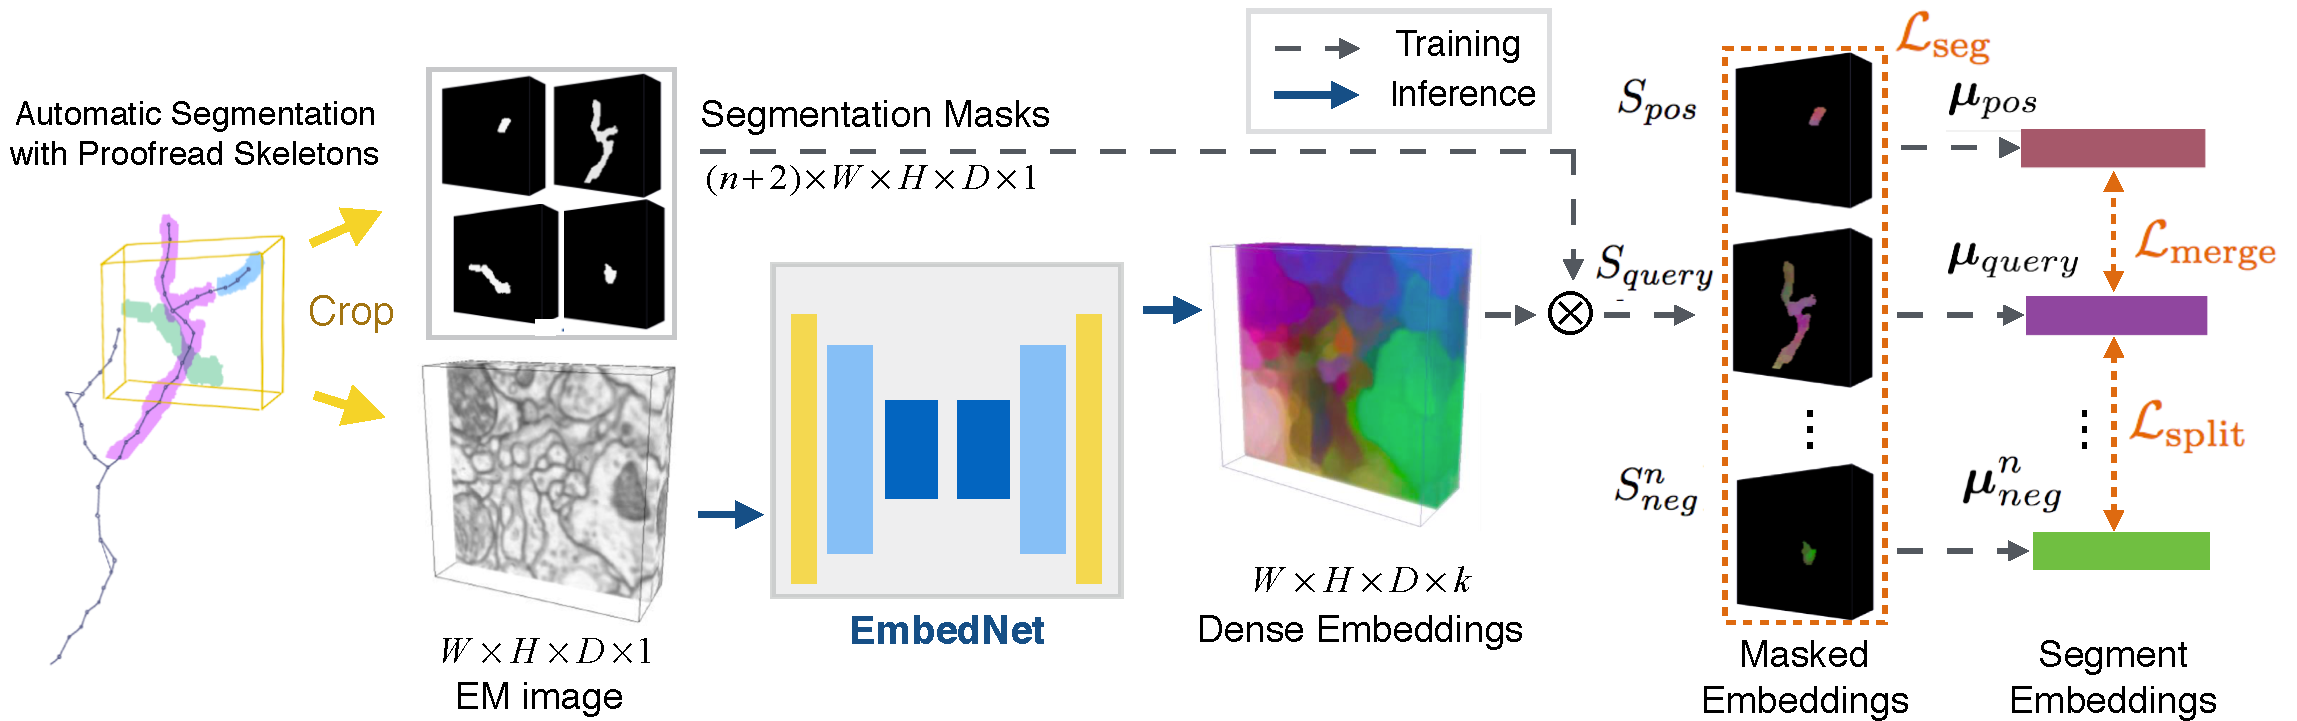
\includegraphics[width=0.88\textwidth]{figs/main.pdf}
    \caption{Our volumetric image embedding network. For a pair of adjacent segments, a small EM volume centered at the truncation point is cropped and fed into EmbedNet to extract per-voxel $k$-dimensional embeddings. The EmbedNet is trained via a contrastive loss based on the pairwise segment connectivity of the query segment and the other neighboring segments.}% 
    \label{fig:embedding}
\end{figure*}


\subsubsection{3D Morphological Representation of Segments.}
The geometric property of segments provides rough clues for connection. For instance, certain patterns like L-shaped or arrow-shaped junctions are uncommon neuronal structures. 
There are several 3D representation forms for expressing segment morphology. For example, EdgeNetwork \cite{matejek2019biologically} uses volumetric masks for segments and applies 3D convolutional neural network (3DCNN) to encode the segment morphology. 
Each voxel carries three labels indicating whether it belongs to segments $S_a$, $S_b$, and $S_a \cup S_b$ respectively. Besides the 3D segment masks, we also explore the surface point cloud as a more efficient morphology representation. Unlike 3DCNNs that apply dense operation for both surface voxel and inner voxels of the target segments, point-based models only process sparse surface points. Centering at the truncation point ${\hat{\mathbf{c}}}_{i,j}$ of the segment to trace, we crop a 3D volume and extract the segment section contours on each image slice and collect all the contour points to compose a point cloud. 
Each point $\mathbf{p}=(x,y,z, id)$, where $(x,y,z)$ refer to the physical coordinate and $id\in\{0,1\}$ signifies surface points from whether $S_a$ or $S_b$. 
The point clouds are further downsampled by farthest point sampling (FPS) to a fixed number of points and normalized in a unit cube. We employ PointNet++ \cite{PointNet++-NIPS-2017} as the morphological feature encoder and connectivity prediction model for the point cloud inputs.

\subsubsection{Fusing Image Features with 3D Representations.}
The segment shape might be distorted due to image distortions (e.g. misalignment between adjacent EM sections) and segmentation errors. Consequently, human tracers rely on the original EM images as the decisive evidence. Sometimes the evidence could lie on just a few voxels. Therefore, we design an image embedding network called EmbedNet to generate delicate and discriminative features for every voxel. From a local EM image cube, our EmbedNet extracts a $k$-dimensional image feature vector for each voxel. To predict the segment connectivity, the image features are integrated with the point geometric features or voxel masks optionally, as illustrated in Fig. \ref{fig:3Dmodel}. 
For the volume representation, the segment masks and image embedding vectors are concatenated directly voxel by voxel. 
Regarding the surface point cloud, we use the average embedding vectors in a $7 \times 7 \times 3$ neighborhood of each point $\mathbf{p}$ as its local image embedding $\mathbf{e}(\mathbf{p})$.
The $k$-D average embedding feature is then concatenated to $(x,y,z,id)$ of each surface point.

 
\subsubsection{Learning Volumetric Image Embedding.} 
\label{Sec:learn-embedding}
%
To learn the image feature representations, we follow the typical supervised contrastive learning framework~\cite{lee2021learning,de2017semantic,zhou2022rethinking} with a contrastive loss that encourages close embeddings between connected segments and distinct embeddings of segments from different neurons.
Fig.~\ref{fig:embedding} shows the pipeline of our EM image embedding learning. 
%
Existing dense embedding learning methods for segmentation usually apply a loss that mainly consists of two parts: intra-cluster variance that measures the deviation of the embeddings of all segment voxels from the cluster center and inter-cluster distance that forces distinct clusters.
In comparison, we focus more on segment-level connectivity rather than voxel-wise segmentation.  
Consequently, we design a novel segment connectivity-oriented contrastive loss to enforce the similarity of the mean embeddings between segments belonging to the same neuron.
 

Our connectivity-oriented contrastive loss consists of a merge loss for positive pairs and a split loss for negative pairs. 
As shown in Fig.~\ref{fig:embedding}, assuming we have a positive connection pair that contains a query segment $S_{query}$ and a positive segment $S_{pos}$ from the same neuron, we crop an EM cube with the over-segmentation masks. Then $n$ segments $\{S_{neg}^1,...,S_{neg}^n\}$ are randomly sampled from adjacent areas to form negative connection pairs with $S_{query}$ and $S_{pos}$ respectively. 
As the EmbedNet extracting per-voxel image embedding feature $\mathbf{e}$, for each segment that contains $M$ voxels within the cropped cube, we compute the mean embedding feature as the segment embedding: $\bm{\mu} = \frac{1}{M} \sum^{M}_{i=1} \mathbf{e}_i$. 
%
Then the merge loss and split loss are computed by:
\begin{equation}
    \begin{aligned}
     \mathcal{L}_{\text {merge }} &=\left\|\bm{\mu}_{query}-\bm{\mu}_{pos}\right\|^2, \\
     \mathcal{L}_{\text {split}} &=\frac{1}{n}\sum_{i=1}^n\max \left(2 \delta_d-\left\|\bm{\mu}_{query}-\bm{\mu}_{neg}^i\right\|, 0\right)^2 \\
    & + \frac{1}{n} \sum_{i=1}^n\max \left(2 \delta_d-\left\|\bm{\mu}_{pos}-\bm{\mu}_{neg}^i\right\|, 0\right)^2.
    \end{aligned}
\end{equation}

This design enables our EmbedNet to make use of the large-scale pairwise connection dataset and learn robust features against diverse imaging quality. 
However, the learning of dense embedding is difficult to converge with only sparse segment-level connectivity supervision. Therefore, we following existing segmentation-based embedding methods to further encourage the embedding to form compact clusters within each segment. 
Without dense segmentation annotations for each complete neuron, which are expensive to manually label for a large-scale dataset with diverse image characteristics, we use the automatic over-segmentation results of EM images as pseudo-segmentation masks and adopt the segmentation clustering loss defined in \cite{lee2021learning}:
\begin{equation}
\label{eq:segmentation-loss}
    \mathcal{L}_{seg} = \mathcal{L}_{\mathrm{int}} + \mathcal{L}_{\mathrm{ext}} + \gamma\mathcal{L}_{\mathrm{reg}},
\end{equation}
%
where $\gamma=0.001$.


The overall loss is composed of the segment connectivity contrastive loss and the voxel segmentation clustering loss:
\begin{equation}\label{eq:overall-loss}
        \mathcal{L}_{\text {total }} = \lambda_1  \mathcal{L}_{\text {merge }} + \lambda_2 \mathcal{L}_{\text {split}} + \lambda_3 \mathcal{L}_{\text {seg}}.
\end{equation}
%
During training, we use $\lambda_1=0.1$, $\lambda_2=1$ and $\delta_d=1.5$. Since $\mathcal{L}_{\text {seg}}$ is contradictory with $\mathcal{L}_{\text {merge}}$, we initialize $\lambda_3$ to $1$ and linearly decrease it to $0.2$.
 

